\newcommand{\ClassPath}{../../VIU_TFM_LaTeX_template}
\documentclass{\ClassPath/viu-tfm-template}
\usepackage{multicol}

\definecolor{maincolor}{HTML}{e65218}

%--------------------------------------------------------------------------
% Definiciones necesarias Modifica con tus datos
%--------------------------------------------------------------------------
\def\nombre{Gómez Olivencia, Rubén}
\def\dni{78910013-A}
\def\titulo{Prototipado y diseño de navegación \linebreak\linebreak\linebreak para la Asociación Internacional de Chefs}
\def\titulacion{Máster Universitario en Desarrollo de Aplicaciones y Servicios Web}
\def\curso{2022-2023}

%Los siguientes son opcionales: si no se ponen, la portada cambia un poco. Ideal para escribir artículos/trabajos cortos
\def\dirige{}
\def\convocatoria{}
\def\asignatura{Ingeniería Software Web}


% importar fichero de Bibliografía
%\addbibresource{Actividad_3.bib}

\begin{document}
    \graphicspath{{../../VIU_TFM_LaTeX_template/}}

    \coverpage

    \tableofcontents

\chapter{Introducción}
A lo largo de este documento se van a analizar los modelos concretos y las decisiones tomadas para la creación de los prototipos y diseños de navegación para la aplicación web creada para la Asociación Internacional de Chefs \textbf{AIC}.

Este documento es una continuación de un documento previo en el que se explicaba el análisis y diseño de la aplicación, por lo que varias de las decisiones aquí tomadas tienen origen en dicho documento previo.


\chapter{Justificación}
Una vez realizado el análisis de requisitos del cliente, habiendo conocido las funcionalidades mínimas que requiere y habiendo obtenido los requisitos funcionales, transaccionales, de interfaz y no funcionales, es momento de comenzar con el prototipado y el diseño de navegación que tendrá finalmente la aplicación web.

\section{Prototipos}
Debemos tener claro que un \textbf{prototipo} es una representación (o simulación) del sistema que se ha planificado y que puede contener las siguientes características:

\begin{itemize}
    \item Interfaz de usuario.
    \item Funcionalidades de entrada y salida.
    \item Todos los usuarios deben entender lo que se muestra en el prototipo.
\end{itemize}

Las ventajas de creación de los prototipos es que al ser un paso previo a la creación de la aplicación, podemos obtener una reacción directa del cliente y sus impresiones, ya que es probable que no entienda las especificaciones de requisitos creadas en el documento anterior. Es decir, la creación de prototipos nos va a dar un \textit{feedback} del cliente de manera rápida y sencilla.

Con los prototipos, no sólo vamos a obtener una respuesta al análisis creado previamente, sino que que durante las pruebas, nos pueden aparecer comportamientos no previstos previamente y por tanto cuestiones a modificar antes de realizar la programación de la aplicación. Este punto \textbf{nos puede ahorrar mucho tiempo y complicaciones que podrían surgir en el futuro}.

Por supuesto hay que entender que existen distintos tipos de creación de prototipos y dependiendo de la cantidad de funcionalidades añadidas al mismo pueden ser más fieles al resultado final. Es por ello que a continuación se especificará el tipo de prototipo creado.


\section{Prototipo creado}

A la hora de crear el prototipo para la aplicación de la \textbf{AIC} se ha optado por las siguientes características:

\vspace{-1em}
\begin{itemize}
    \item \textbf{Fidelidad alta}: Se ha querido crear un conjunto de pantallas que le van a proporcionar a los responsables de la \textbf{AIC} un modelo dinámico que pueden utilizar para entender cómo va a ser el resultado final.

    De esta manera, podrán dar el visto bueno a distintos apartados (como pueden ser los colores, las fuentes tipográficas utilizadas, la disposición de algunos componentes) antes de comenzar con el apartado de programación.

    \item \textbf{Uso específico}: Se ha optado por la creación de un prototipo operacional que se ha ido refinando en distintas iteraciones a medida que se iban añadiendo funcionalidades requeridas por el cliente. De esta manera, y tal como se ha dicho previamente, se han encontrado comportamientos no previstos que se han mejorado de cara a que durante la etapa de desarrollo no se pierda el tiempo.

    \item \textbf{Detalle y cantidad de funcionalidades}: Teniendo en cuenta el tipo de aplicación que quiere la \textbf{AIC}, ha sido posible generar un prototipo llamado “diagonal”. Esto quiere decir que se han modelado muchas características del sistema y con gran cantidad de detalle. Esto ha sido posible gracias a que \textbf{gran parte de las funcionalidades se han modularizado y estas se han podido reutilizar} a lo largo de distintas pantallas.

    \item \textbf{Ejecutabilidad}: El prototipo creado se puede considerar que es un \textbf{prototipo interactivo} ya que responde a ciertas entradas que realiza el usuario pero bien es cierto que al no disponer de un servicio de \textit{backend}, dichas funcionalidades siempre son las mismas.
\end{itemize}

Con todo ello, se ha conseguido que los responsables de la \textbf{AIC} hayan dado una retroalimentación, que hasta ahora no había sido posible, que se haya tenido en cuenta esa información para mejorar el propio prototipo y que se tendrá en cuenta durante la etapa de desarrollo de la aplicación.

A modo de resumen, el prototipo creado es un \textbf{prototipo del sistema completo} en el que se pueden visualizar, y con el que se puede interactuar para ver las distintas funcionalidades que tendrá la aplicación final. De nuevo, destacar que al no contar con un sistema de \textit{backend}, el registro de usuarios o de recetas no va a funcionar (no se guardan los datos), pero todo el proceso es igual al que será en el resultado final.

El prototipo se puede visualizar, e interactuar con él, en la siguiente  \href{https://yuki.github.io/VIU_03MASW/preview.html}{dirección web}.


\chapter{Modelos concretos}

A continuación se van a detallar los modelos concretos de las distintas funcionalidades que tiene el prototipo creado, y que posteriormente será desarrollado en la aplicación web.

A continuación se puede ver la página principal de la web:

\begin{center}
    \vspace{-10pt}
    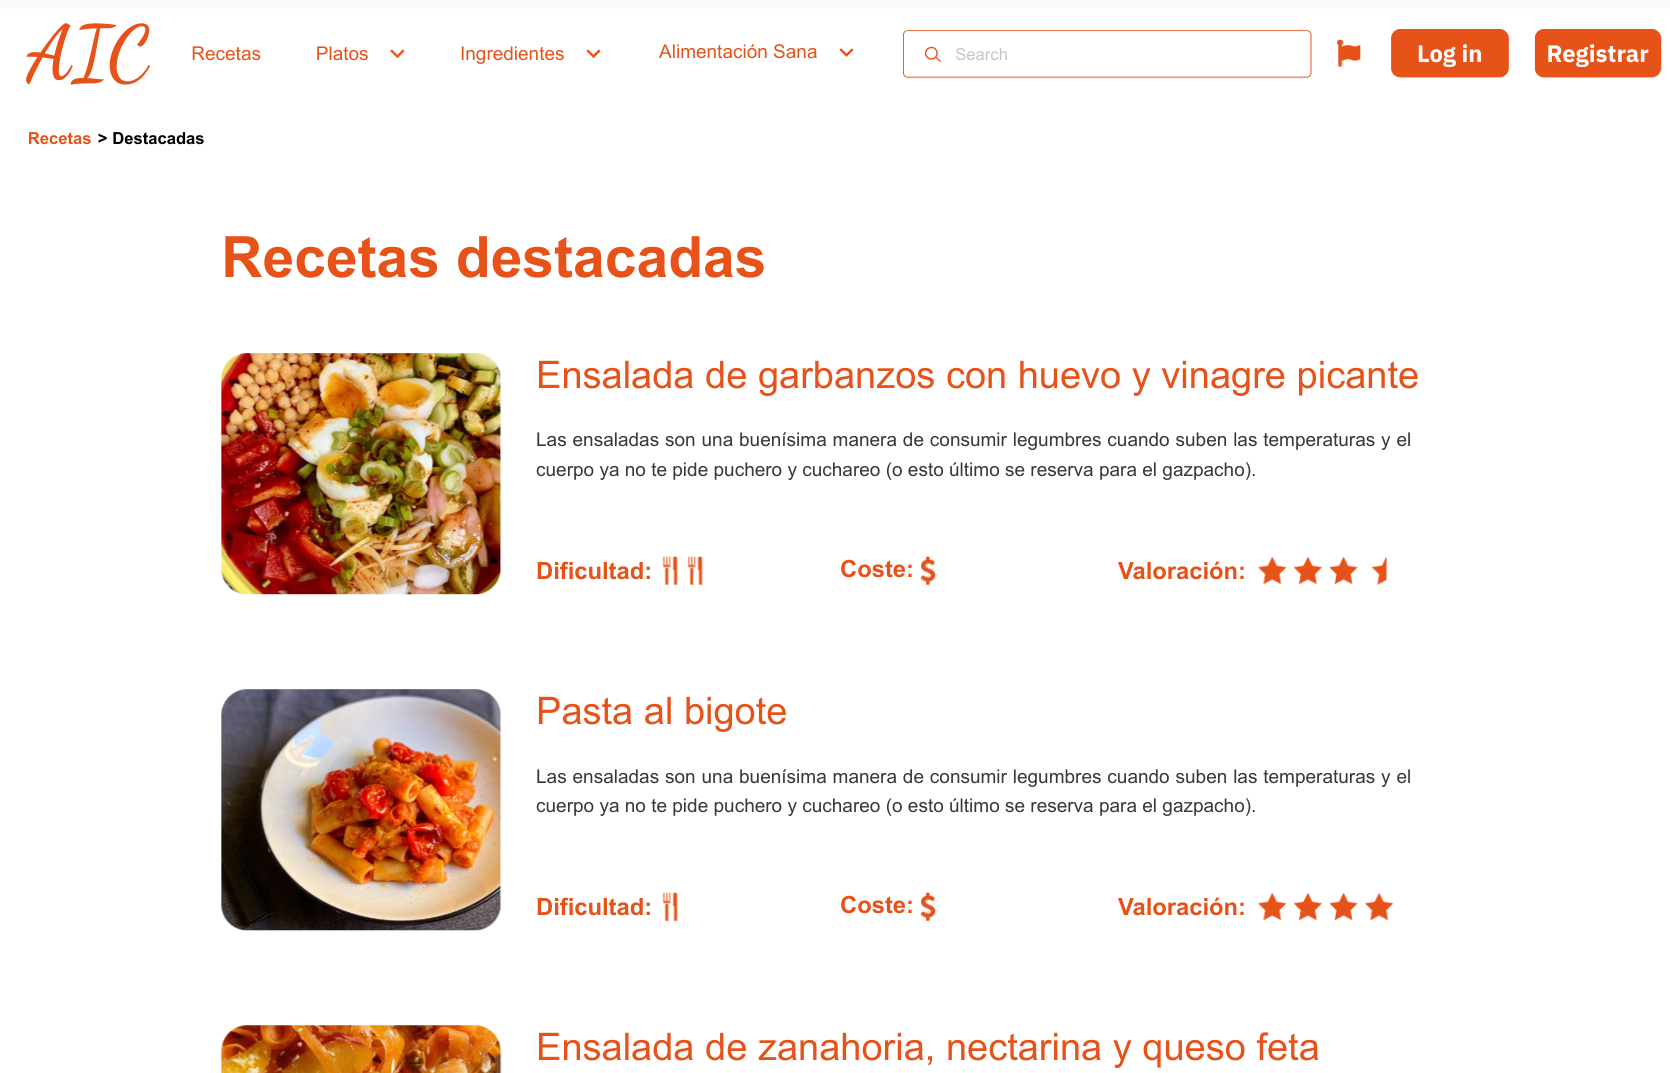
\includegraphics[frame,width=0.7\linewidth]{img/aic/0_general.png}
    \vspace{-20pt}
\end{center}

Tal como se ha dicho previamente, todo lo aquí expuesto se puede ver e interactuar a través de la siguiente \href{https://yuki.github.io/VIU_03MASW/preview.html}{dirección web}, que a su vez después también se representará a través de los esquemas de organización.


\section{Menú principal}

La aplicación web cuenta con un menú en la parte superior que es el punto de partida para que el usuario pueda acceder a distintos apartados del portal. A continuación una imagen del menú:

\begin{center}
    \vspace{-10pt}
    
\includegraphics[frame,width=0.9\linewidth]{img/aic/0_menu.png}
    \vspace{-20pt}
\end{center}

Como se puede ver, se pueden diferenciar distintas “columnas” que son secciones a los que el usuario puede acceder haciendo uso del ratón. A continuación se detallan cada uno de ellos:

\vspace{-1em}
\begin{itemize}
    \item \textbf{Logotipo de AIC}: Para que se reconozca la web en la que nos encontramos, se ha añadido el logo de la \textbf{AIC}. Al hacer click sobre él se irá a la web principal de la aplicación web.
    \item \textbf{Recetas}: Es el reclamo principal del portal, la sección de recetas. Al hacer click sobre este apartado iremos a las “recetas destacadas” que pueden ser las últimas introducidas o un aleatorio de las mismas.

    \item \textbf{Platos}: Es un menú desplegable con las categorías de los distintos tipos de platos que existen diferenciados en la aplicación. Al hacer click se despliega el menú en el que se podrá elegir la categoría que interese al usuario. Al elegir uno, se irá a un listado de recetas de dicha categoría.

    \item \textbf{Ingredientes}: Igual que el caso anterior, pero con los ingredientes. Un desplegable en el que aparecen categorizadas por familias los ingredientes que pueden ser seleccionados. Al elegir una familia de ingredientes se irá a un listado de recetas que contiene dicha familia de ingredientes.

    \item \textbf{Alimentación sana}: Es un menú en el que se puede seleccionar la nueva información que la \textbf{AIC} ha querido incorporar en la aplicación acerca de la alimentación sana.

    \item \textbf{Caja de búsqueda}: Es un cajón de búsqueda en el que el usuario podrá introducir nombre de recetas, ingredientes, tipos de platos o palabra que puede contener una receta. Al introducir las palabras y darle a “intro” se irá a la web de resultados.

    \item \textbf{Selección de idioma}: Mediante el uso del icono de una bandera, se puede modificar el idioma en el que se encuentra el portal web.

    \item \textbf{Botón de “\textit{login}”}: Para realizar la autenticación del usuario y contraseña que tenga el usuario.

    \item \textbf{Botón de “registrar”}: Para aquellos usuarios que quieran introducir recetas nuevas, deben registrarse previamente a través de este botón.
    \vspace{-1em}
\end{itemize}

Es importante destacar que cuando un usuario se ha autenticado en la plataforma el menú cambia apareciendo en lugar de los botones de “Log in” y “Registrar” el menú contextual del usuario.

Todas estas secciones serán explicadas de manera detallada en las siguientes secciones y en el mapa de navegación.

\section{Camino recorrido por el usuario}

Debajo del menú, y con intención de que el usuario sepa en todo momento dónde se encuentra, aparece el “camino recorrido” de la situación actual.

\begin{center}
    \vspace{-10pt}
    \textbf{\color{maincolor}Alimentación sana > \space Ingredientes \color{black} >\space Carnes}
    \vspace{-15pt}
\end{center}

Teniendo en cuenta el uso de colores, también se identifican que las dos primeras palabras son enlaces que llevará al usuario a dichas secciones, mientras que el último apartado (en color negro), es el sitio actual donde se encuentra el usuario.


\section{Registro de usuario}
Tal como se ha dicho previamente, y tal como aparecen en los requisitos funcionales del documento anterior, para que un usuario pueda registrar una receta debe estar registrado en el sistema. Para que un usuario se pueda registrar debe hacer click sobre el botón “Registrar” del menú y acto seguido le aparecerá la siguiente pantalla:

\begin{center}
    \vspace{-10pt}
    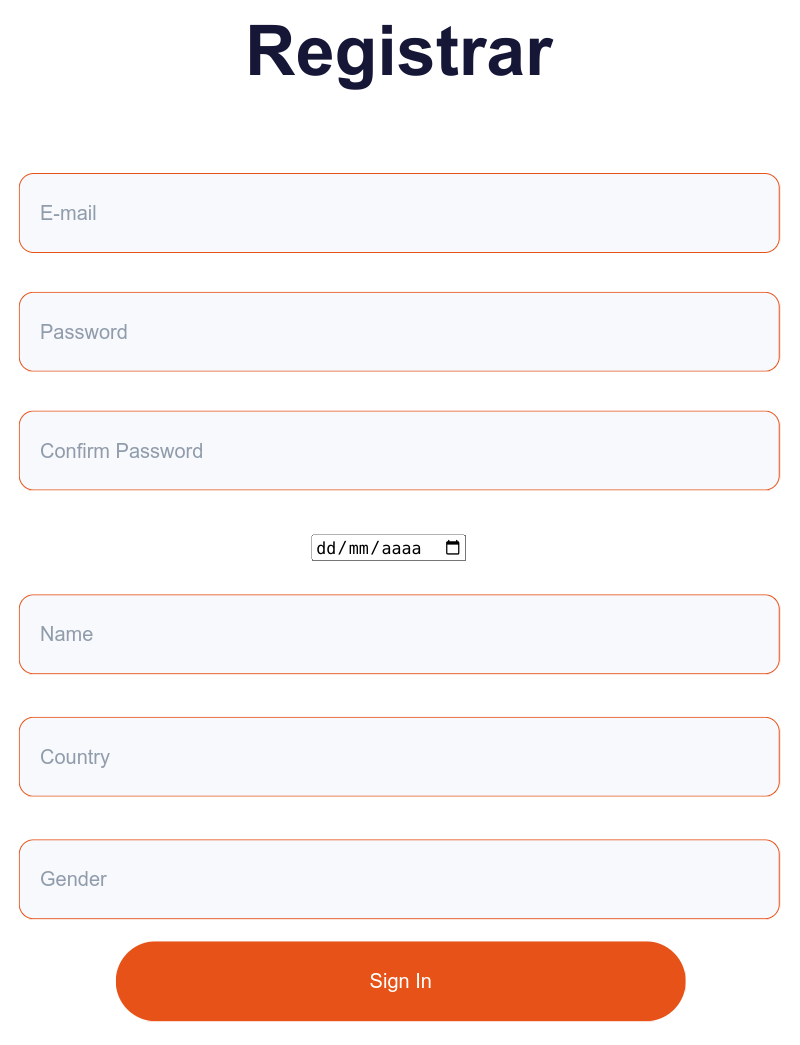
\includegraphics[frame,width=0.4\linewidth]{img/aic/registro.png}
    \vspace{-20pt}
\end{center}

Al llegar a esta pantalla, se deberán rellenar los datos y pulsar el botón para que posteriormente el usuario esté registrado en la aplicación y a partir de ahí se puedan registrar recetas.


\section{Autenticación de usuario}
Una vez el usuario ya esté registrado, si no aparece como “logueado”, el usuario deberá darle al botón de “Log in” del menú para poder autenticarse en la aplicación. Al dar a dicho botón le aparecerá la siguiente pantalla:

\begin{center}
    \vspace{-10pt}
    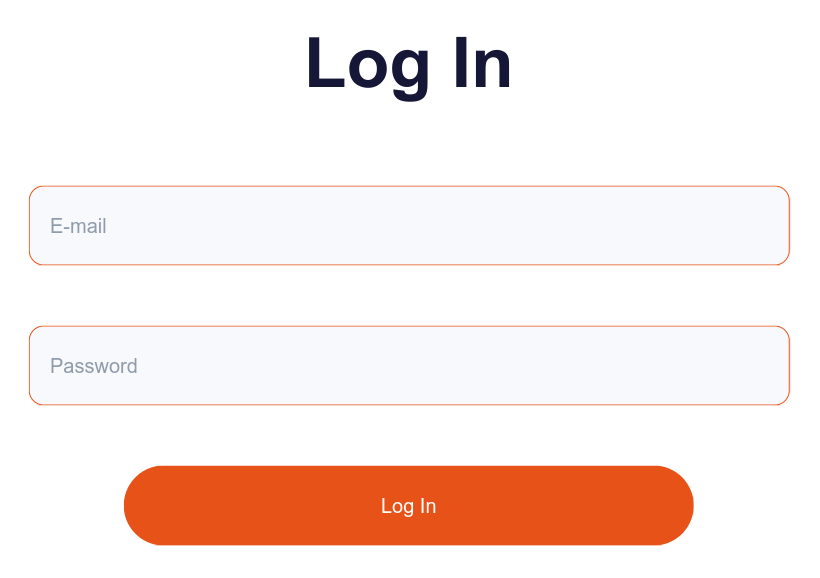
\includegraphics[frame,width=0.4\linewidth]{img/aic/login.png}
    \vspace{-20pt}
\end{center}

El usuario deberá introducir el \textit{e-mail} con el que se registró y la contraseña utilizada.

Cuando un usuario se ha autenticado, el menú principal de la aplicación cambia, desapareciendo los botones de autenticación y registro para que en su lugar aparezca lo siguiente:


\begin{center}
    \vspace{-10pt}
    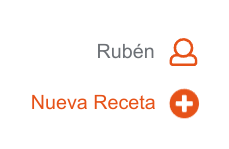
\includegraphics[frame,width=0.3\linewidth]{img/aic/logueado.png}
    \vspace{-20pt}
\end{center}

En este caso lo que aparece es el nombre del usuario, que a su vez es un desplegable, y un enlace para registrar nuevas recetas. El menú del usuario cuenta con:


\begin{multicols}{2}
    \begin{center}
        \vspace{-10pt}
        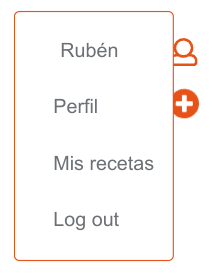
\includegraphics[width=0.8\linewidth]{img/aic/logueado_menu.png}
        \vspace{-20pt}
    \end{center}

   \begin{itemize}
       \item \textbf{Nombre de usuario}: El nombre del usuario autenticado.
       \item \textbf{Perfil}: Página donde podrá modificar su contraseña, nombre, e-mail, ...
       \item \textbf{Mis recetas}: Página donde podrá ver las recetas que ha registrado.
       \item \textbf{Log out}: Opción para dejar de estar autenticado en la plataforma.
   \end{itemize}
\end{multicols}

Todas estas opciones, como ya se ha dicho, sólo aparecen cuando el usuario está autenticado.


\section{Registrar nueva receta}

Cuando un usuario quiere registrar una nueva receta, primero debe estar autenticado como hemos visto en el punto anterior. Al hacer click sobre “{\color{maincolor}Nueva Receta}” aparecerá una nueva página donde se podrá registrar una nueva receta.

A la hora de registrar una nueva receta, habrá que añadir distintos apartados tal como aparecen en las imágenes siguientes:


    \begin{center}
        \vspace{-10pt}
        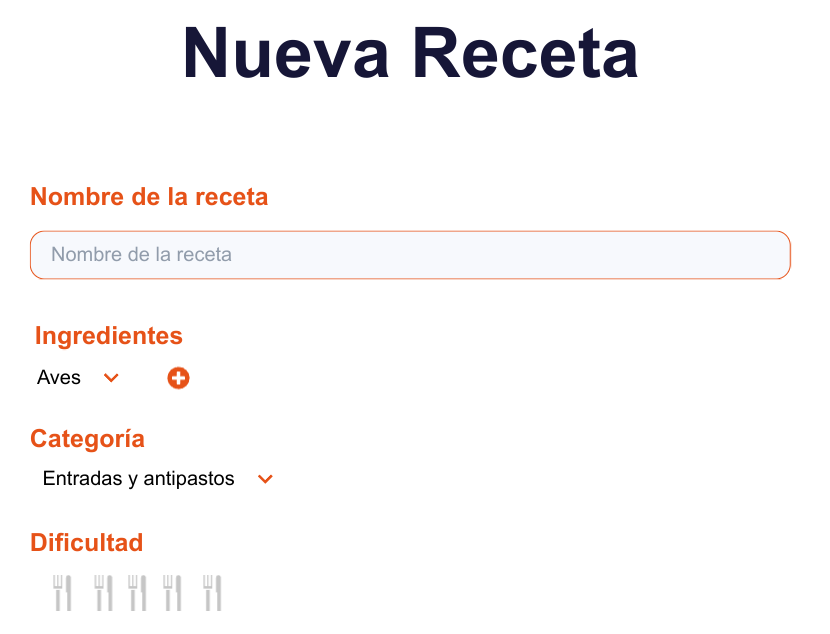
\includegraphics[width=0.6\linewidth]{img/aic/nueva_receta_1.png}
        \vspace{-20pt}
    \end{center}

    \begin{center}
        \vspace{-10pt}
        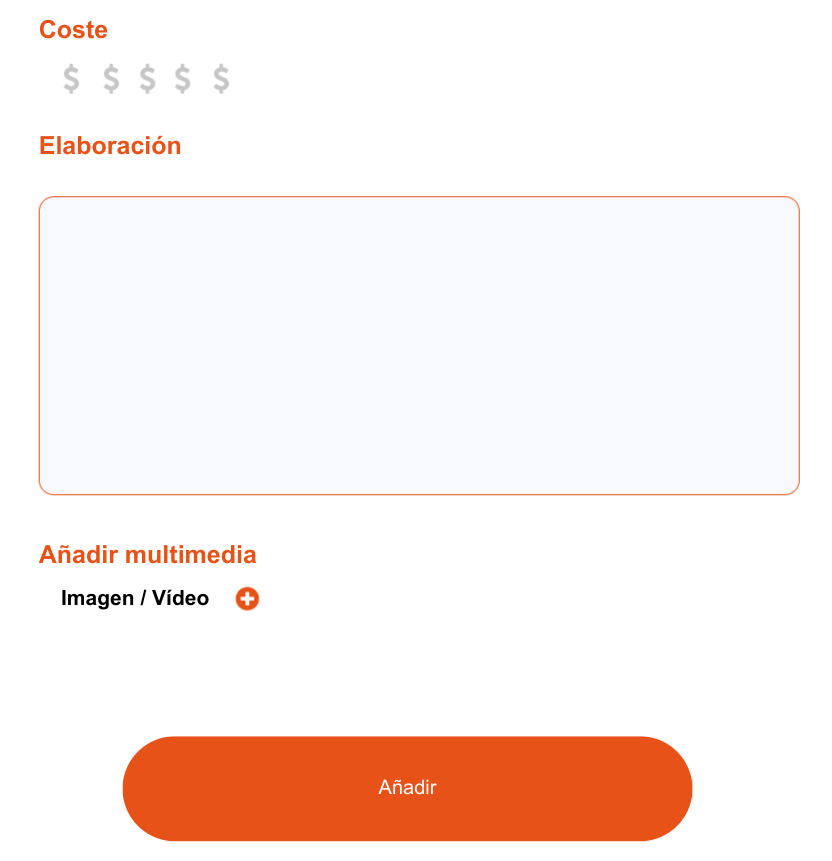
\includegraphics[width=0.6\linewidth]{img/aic/nueva_receta_2.png}
        \vspace{-20pt}
    \end{center}

Tal como se puede ver, los apartados son:

\begin{itemize}
    \item \textbf{Nombre de la receta}: Un nombre que identifique la receta.
    \item \textbf{Ingredientes}: Es un menú desplegable junto con un icono de “+” que permitirá añadir tantos ingredientes como tenga la receta.
    \item \textbf{Categoría}: Es un menú desplegable para elegir una única categoría del plato de los requisitos indicados en el documento anterior.
    \item \textbf{Dificultad}: Para indicar la dificultad se ha optado por el uso de iconos con forma de tenedor y cuchillo, que marca de 1 a 5 la dificultad.
    \item \textbf{Coste}: Similar al caso anterior, pero con el símbolo de dolar para indicar el coste.
    \item \textbf{Elaboración}: Campo de texto donde el usuario podrá explicar cómo se realiza la receta.
    \item \textbf{Añadir multimedia}: Para poder añadir imágenes o vídeos de  la elaboración de la receta, se ha añadido dicha opción junto con el icono “+” para poder añadir varios ficheros.
    \item \textbf{Botón Añadir}: Una vez rellenado todos los campos, se debe pulsar el botón añadir.
\end{itemize}


\section{Búsqueda de recetas}




\chapter{Esquema de organización}





\chapter{Mapa de navegación}





\chapter{Conclusiones}




%\printbibliography[title={Referencias bibliográficas},heading=bibintoc]

\end{document}
